\documentclass[compress]{beamer}
\usepackage{irbookslide}
\usepackage{irilmenau2}
\usepackage{tikz}
\usepackage{url}
\usepackage{ifxetex}
%\RequireXeTeX
\usepackage{fontspec} % zahteva paket euenc
\usepackage{xunicode}
\usepackage{xltxtra}
\usepackage{polyglossia}
\usepackage{minted}
\usepackage[noend]{algorithmic}
\renewcommand{\algorithmicrequire}{\textbf{Input:}}
\renewcommand{\algorithmicensure}{\textbf{Output:}}
\renewcommand{\algorithmiccomment}[1]{\hfill \{\myred{#1}\}}
\usepackage{xcolor,colortbl}
\usepackage{textcomp}
\usepackage{unicode-math}
%\setdefaultlanguage[script=Latin]{serbian}


\title{Mape, heš tabele, skip liste, skupovi}
\author{\textcopyright \ \ Goodrich, Tamassia, Goldwasser}
\institute{Katedra za informatiku, Fakultet tehničkih nauka, Univerzitet u
Novom Sadu}
\date{2014.}
\subject{Predavanja sa ASP}

\begin{document}

\frame{\titlepage}

\section[Mapa]{Mapa}
\begin{frame}[fragile]
  \frametitle{Mapa}
  \begin{itemize}
    \item Pythonov rečnik (klasa \textbf{dict}) preslikava \textbf{ključeve} na \textbf{vrednosti} 
    \item drugo ime: \myred{asocijativni niz} ili \myred{mapa}
    \item ključevi su jedinstveni (nema ponavljanja)
    \item vrednosti ne moraju biti jedinstvene
  \end{itemize}
  \begin{center}
    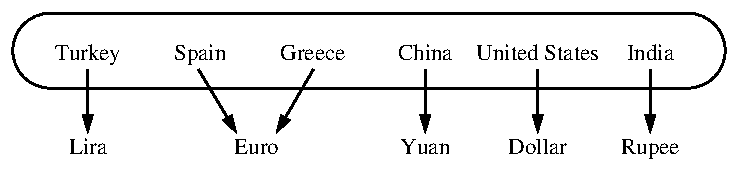
\includegraphics[width=10cm]{asp-10-pic01.pdf}
  \end{center}
\end{frame}

\begin{frame}[fragile]
  \frametitle{Mapa ATP: osnovne operacije}
  \begin{center}
    \begin{tabular}{rp{8cm}}
      \textbf{\texttt{M[k]}} & vraća vrednost $v$ vezanu za ključ $k$ u mapi $M$; ako ne postoji, izaziva \texttt{KeyError}; implementira je \texttt{\_\_getitem\_\_} \\ \hline
      \textbf{\texttt{M[k] = v}} & dodeljuje vrednost $v$ ključu $k$ u mapi $M$; ako ključ već postoji, zamenjuje staru vrednost; implementira je \texttt{\_\_setitem\_\_} \\ \hline
      \textbf{\texttt{del M[k]}} & uklanja element sa ključem $k$ iz mape $M$; ako ne postoji, izaziva \texttt{KeyError}; implementira je \texttt{\_delitem\_\_} \\ \hline
      \textbf{\texttt{len(M)}} & vraća broj elemenata u mapi $M$; implementira je \texttt{\_\_len\_\_} \\ \hline
      \textbf{\texttt{iter(M)}} & generiše listu \textbf{ključeva} iz mape $M$;  implementira je \texttt{\_\_iter\_\_} \\
    \end{tabular}
  \end{center}
\end{frame}

\begin{frame}[fragile]
  \frametitle{Mapa ATP: dodatne operacije}
  \begin{center}
    \begin{tabular}{rp{6cm}}
      \textbf{\texttt{k in M}} & vraća \texttt{True} ako mapa $M$ sadrži ključ $k$; implementira je \texttt{\_\_contains\_\_} \\ \hline
      \textbf{\texttt{M.get(k, d=None)}} & vraća $M[k]$ ako ključ $k$ postoji u $M$; inače vraća default vrednost $d$; ne izaziva \texttt{KeyError} \\ \hline
      \textbf{\texttt{M.setdefault(k, d)}} & ako $k$ postoji u mapi, vraća $M[k]$; ako ne postoji, postavlja $M[k]=d$ i vraća $d$ \\ \hline
      \textbf{\texttt{M.pop(k, d=None)}} & uklanja element sa ključem $k$ i vraća vezanu vrednost $v$; ako ključ $k$ nije u mapi $M$, vraća $d$ ili izaziva \texttt{KeyError} ako je $d$ jednako \texttt{None}
    \end{tabular}
  \end{center}
\end{frame}

\begin{frame}[fragile]
  \frametitle{Mapa ATP: još malo operacija}
  \begin{center}
    \begin{tabular}{rp{8cm}}
      \textbf{\texttt{M.popitem()}} & uklanja neki element mape i vraća ($k$,$v$); ako je mapa prazna izaziva \texttt{KeyError} \\ \hline
      \textbf{\texttt{M.clear()}} & uklanja sve elemente iz mape \\ \hline
      \textbf{\texttt{M.keys()}} & vraća skup svih ključeva iz $M$ \\ \hline
      \textbf{\texttt{M.values()}} & vraća skup svih vrednosti iz $M$ \\ \hline
      \textbf{\texttt{M.items()}} & vraća skup svih parova ($k$,$v$) iz $M$ \\ \hline
      \textbf{\texttt{M.update(M2)}} & dodeljuje \texttt{M[k]=v} za svaki ($k$,$v$) iz $M2$ \\ \hline
      \textbf{\texttt{M == M2}} & vraća \texttt{True} ako mape sadrže iste parove ($k$,$v$) \\ \hline
      \textbf{\texttt{M != M2}} & vraća \texttt{True} ako mape ne sadrže iste parove ($k$,$v$)
    \end{tabular}
  \end{center}
\end{frame}

\begin{frame}[fragile,shrink]
  \frametitle{Mapa ATP: primer}
  \begin{center}
    \begin{tabular}{lcl}
      \textbf{operacija} & \textbf{rezultat} & \textbf{mapa} \\ \hline
      \texttt{len(M)} & 0 & \texttt{\{ \}} \\
      \texttt{M['K']=2} & -- & \texttt{\{'K':2\}} \\
      \texttt{M['B']=4} & -- & \texttt{\{'K':2, 'B':4\}} \\
      \texttt{M['U']=2} & -- & \texttt{\{'K':2, 'B':4, 'U':2\}} \\
      \texttt{M['V']=8} & -- & \texttt{\{'K':2, 'B':4, 'U':2, 'V':8\}} \\
      \texttt{M['K']=9} & -- & \texttt{\{'K':9, 'B':4, 'U':2, 'V':8\}} \\
      \texttt{M['B']} & 4 & \texttt{\{'K':9, 'B':4, 'U':2, 'V':8\}} \\
      \texttt{M['X']} & \texttt{KeyError} & \texttt{\{'K':9, 'B':4, 'U':2, 'V':8\}} \\
      \texttt{M.get('F')} & \texttt{None} & \texttt{\{'K':9, 'B':4, 'U':2, 'V':8\}} \\
      \texttt{M.get('F', 5)} & \texttt{5} & \texttt{\{'K':9, 'B':4, 'U':2, 'V':8\}} \\
      \texttt{M.get('K', 5)} & \texttt{9} & \texttt{\{'K':9, 'B':4, 'U':2, 'V':8\}} \\
      \texttt{len(M)} & \texttt{4} & \texttt{\{'K':9, 'B':4, 'U':2, 'V':8\}} \\
      \texttt{del M['V']} & -- & \texttt{\{'K':9, 'B':4, 'U':2\}} \\
      \texttt{M.pop('K')} & 9 & \texttt{\{'B':4, 'U':2\}} \\
      \texttt{M.keys()} & \texttt{'B','U'} & \texttt{\{'B':4, 'U':2\}} \\
      \texttt{M.values()} & \texttt{4,2} & \texttt{\{'B':4, 'U':2\}} \\
      \texttt{M.items()} & \texttt{('B',4),('U',2)} & \texttt{\{'B':4, 'U':2\}} \\
      \texttt{M.setdefault('B',1)} & \texttt{4} & \texttt{\{'B':4, 'U':2\}} \\
      \texttt{M.setdefault('A',1)} & \texttt{1} & \texttt{\{'A':1, 'B':4, 'U':2\}} \\
      \texttt{M.popitem()} & \texttt{('B',4)} & \texttt{\{'A':1, 'U':2\}}
    \end{tabular}
  \end{center}
\end{frame}

\begin{frame}[fragile]
  \frametitle{Različite implementacije mape}
  \begin{center}
    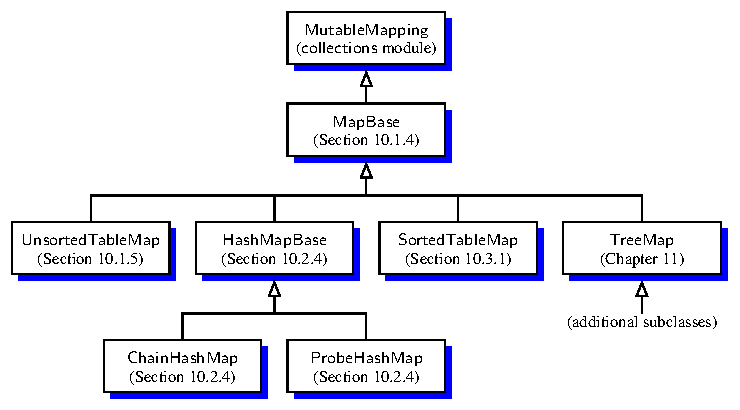
\includegraphics[width=11cm]{asp-10-pic02.pdf}
  \end{center}
\end{frame}

\begin{frame}[fragile,shrink]
  \frametitle{Implementacija MapBase}
\begin{minted}[linenos=false]{python}
from collections import MutableMapping

class MapBase(MutableMapping):
  """Our own abstract base class that includes a nonpublic _Item class."""

  #-- nested _Item class --
  class _Item:
    """Lightweight composite to store key-value pairs as map items."""
    __slots__ = '_key', '_value'

    def __init__(self, k, v):
      self._key = k
      self._value = v

    def __eq__(self, other):               
      return self._key == other._key   # compare items based on their keys

    def __ne__(self, other):
      return not (self == other)       # opposite of __eq__

    def __lt__(self, other):               
      return self._key < other._key    # compare items based on their keys
\end{minted}
\end{frame}

\begin{frame}[fragile]
  \frametitle{Mapa pomoću liste}
  \begin{itemize}
    \item jedna moguća implementacija mape je pomoću dvostruko spregnute liste 
    \item elemente čuvamo u proizvoljnom redosledu
  \end{itemize}
  \begin{center}
    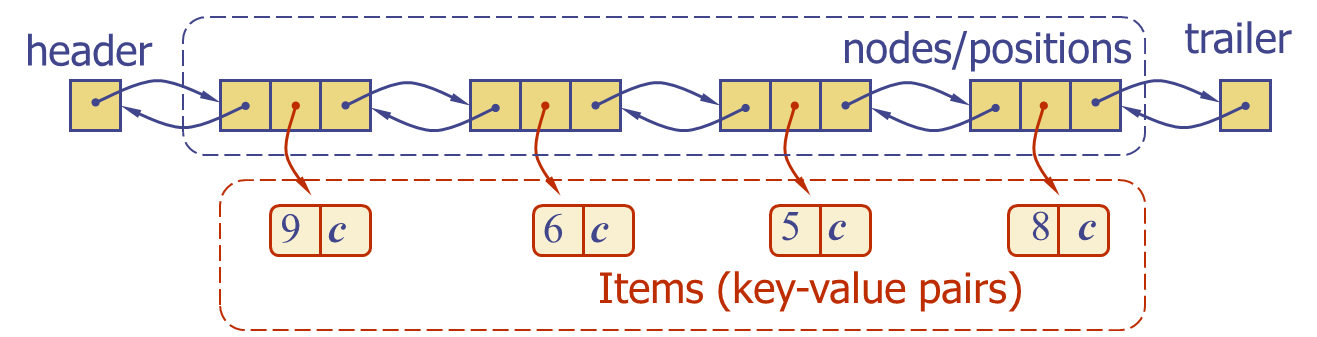
\includegraphics[width=10cm]{asp-10-pic03.png}
  \end{center}
\end{frame}

\begin{frame}[fragile,shrink]
  \frametitle{Mapa pomoću liste: implementacija $_1$}
\begin{minted}[linenos=false]{python}
class UnsortedTableMap(MapBase):
  """Map implementation using an unordered list."""

  def __init__(self):
    """Create an empty map."""
    self._table = []                              # list of _Item's
  
  def __getitem__(self, k):
    """Return value associated with key k (raise KeyError if not found)."""
    for item in self._table:
      if k == item._key:
        return item._value
    raise KeyError('Key Error: ' + repr(k))

  def __setitem__(self, k, v):
    """Assign value v to key k, overwriting existing value if present."""
    for item in self._table:
      if k == item._key:                          # Found a match:
        item._value = v                           # reassign value
        return                                    # and quit    
    # did not find match for key
    self._table.append(self._Item(k,v))
\end{minted}
\end{frame}

\begin{frame}[fragile,shrink=25]
  \frametitle{Mapa pomoću liste: implementacija $_2$}
\begin{minted}[linenos=false]{python}
  def __delitem__(self, k):
    """Remove item associated with key k (raise KeyError if not found)."""
    for j in range(len(self._table)):
      if k == self._table[j]._key:                # Found a match:
        self._table.pop(j)                        # remove item
        return                                    # and quit    
    raise KeyError('Key Error: ' + repr(k))

  def __len__(self):
    """Return number of items in the map."""
    return len(self._table)

  def __iter__(self):                             
    """Generate iteration of the map's keys."""
    for item in self._table:
      yield item._key                             # yield the KEY
\end{minted}
\end{frame}

\begin{frame}[fragile]
  \frametitle{Mapa pomoću liste: performanse}
  \begin{itemize}
    \item \textbf{dodavanje} traje $O(1)$ -- novi element možemo dodati na početak ili na kraj  
    \item \textbf{traženje} ili \textbf{uklanjanje} traje $O(n)$ -- u najgorem slučaju (nije pronađen element) mora se proći kroz celu listu
    \item ovakva implementacija je korisna samo za mape sa malim brojem elemenata
    \item ili ako je dodavanje najčešća operacija, dok se traženje i uklanjanje retko obavljaju
  \end{itemize}
\end{frame}

\section[Hash tabela]{Hash tabela}
\begin{frame}[fragile]
  \frametitle{Hash tabela}
  \begin{itemize}
    \item mapa omogućava pristup korišćenjem \textbf{ključeva} kao \textbf{indeksa} -- \texttt{M[k]}  
    \item zamislimo mapu koja kao ključeve korisiti cele brojeve iz intervala $[0, N-1]$ za neko $N > n$
    \item za čuvanje elemenata možemo koristiti \myred{lookup} niz dužine $N$
    \item npr. mapa sa elementima $(1,D), (3,Z), (6,C), (7,Q)$
  \end{itemize}
  \begin{center}
    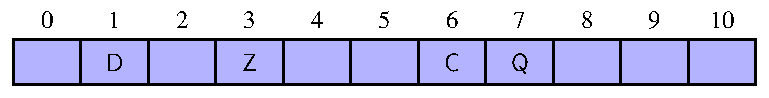
\includegraphics[width=10cm]{asp-10-pic04.pdf}
  \end{center}
  \begin{itemize}
    \item operacije su $O(1)$  
  \end{itemize}
\end{frame}

\begin{frame}[fragile]
  \frametitle{Hash tabela}
  \begin{itemize}
    \item šta ako je $N >> n$ ?  
    \item šta ako ključevi nisu celi brojevi?
    \item pretvorićemo ključeve u cele brojeve pomoću \myred{hash funkcije}
    \item dobra hash funkcija će ravnomerno distribuirati ključeve u $[0,N-1]$
    \item ali može biti duplikata
    \item duplikate ćemo čuvati u ,,kantama`` -- tzv. \myred{bucket array}
  \end{itemize}
  \begin{center}
    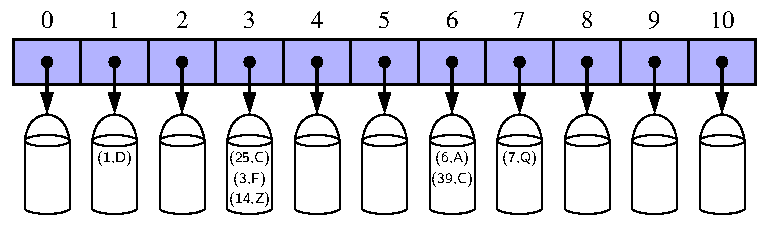
\includegraphics[width=10cm]{asp-10-pic05.pdf}
  \end{center}
\end{frame}

\begin{frame}[fragile]
  \frametitle{Hash funkcija}
  \begin{itemize}
    \item \textbf{hash funkcija} mapira ključeve na indekse u hash tabeli  
    \item npr. poslednje četiri cifre broja telefona
  \end{itemize}
  \begin{center}
    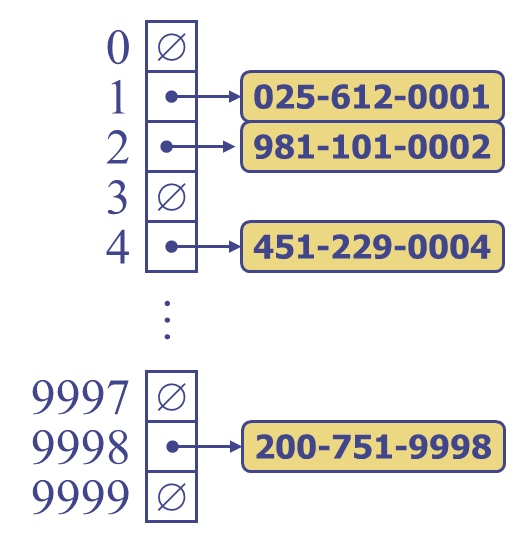
\includegraphics[width=4cm]{asp-10-pic06.png}
  \end{center}
\end{frame}

\begin{frame}[fragile]
  \frametitle{Hash funkcija}
  \begin{itemize}
    \item \textbf{hash funkcija} mapira ključ $k$ na ceo broj u intervalu $[0,N-1]$
    \item gde je $N$ kapacitet niza kanti $A$
    \item element $(k,v)$ čuvamo u nizu kao $A[h(k)]$
    \item \myred{kolizija}: dve vrednosti ključa koje daju isti hash
    \item dobre hash funkcije imaju \textbf{vrlo malo} kolizija
  \end{itemize}
\end{frame}

\begin{frame}[fragile]
  \frametitle{Hash funkcija}
  \begin{itemize}
    \item često se hash funkcija može posmatrati kao kompozicija dve funkcije:
    \item \myred{hash code}: mapira ključ na ceo broj
    \item \myred{compression function}: mapira hash kôd na broj u intervalu $[0,N-1]$ 
  \end{itemize}
  \begin{center}
    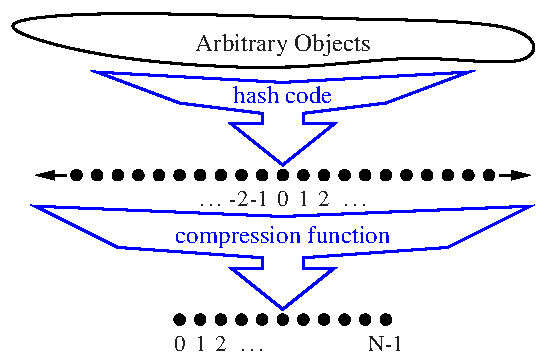
\includegraphics[width=7cm]{asp-10-pic07.pdf}
  \end{center}
\end{frame}

\begin{frame}[fragile]
  \frametitle{Hash funkcija}
  \begin{itemize}
    \item ako se hash funkcija posmatra kao \\ \myred{hash code} $\circ$ \myred{compression function}
    \item tada hash code ne zavisi od veličine niza kanti \\ \ \\
    \item vrednosti koje su ,,blizu`` u skupu ključeva ne moraju imati hasheve koji su ,,blizu`` 
  \end{itemize}
\end{frame}

\begin{frame}[fragile]
  \frametitle{Hash code $_1$}
  \begin{itemize}
    \item memorijska adresa
    \begin{itemize}
      \item adresa Python objekta u memoriji kao hash code
      \item dobro osim za numeričke tipove i stringove
    \end{itemize}
    \item integer cast 
    \begin{itemize}
      \item za svaki tip podataka koji se predstavlja sa najviše onoliko bita koliko i \textbf{int} možemo uzeti int interpretaciju njegovih bita
      \item za tipove koji zauzimaju više memorije moramo nekako ,,sažeti`` njegove bite
      \item npr. \textbf{float} broj u Pythonu zauzima 64 bita a hash kod 32; možemo izabrati
      \begin{itemize}
        \item gornjih 32 bita
        \item donjih 32 bita
        \item neku kombinaciju sva 64 bita: XOR ili zbir gornje i donje polovine, itd.
      \end{itemize}
    \end{itemize}
  \end{itemize}
\end{frame}

\begin{frame}[fragile]
  \frametitle{Hash code $_2$}
  \begin{itemize}
    \item suma komponenti
    \begin{itemize}
      \item podelimo bitove ključa na delove po 32 bita
      \item saberemo delove (ignorišemo overflow)
      \item zgodno za numeričke ključeve duže od int-a
    \end{itemize}
    \item polinomska akumulacija
    \begin{itemize}
      \item podelimo bitove ključa na delove fiksne dužine (npr. 8, 16, 32 bita) $a_0 a_1 a_2 \ldots a_{n-1}$
      \item izračunamo polinom (ignorišući overflow) za fiksno $z$:
      $$ p(z) = a_0 + a_1 z + a_2 z^2 + \ldots + a_{n-1} z^{n-1}$$
    \end{itemize}
  \end{itemize}
\end{frame}

\begin{frame}[fragile]
  \frametitle{Hash code $_3$}
  \begin{itemize}
    \item polinomska akumulacija
    \begin{itemize}
      \item posebno zgodno za stringove ($z=33$ daje samo 6 kolizija za 50.000 engleskih reči)
      \item polinom $p(z)$ se može izračunati u $O(n)$ vremenu Hornerovom metodom
      \begin{itemize}
        \item sledeći polinomi se računaju u $O(1)$ vremenu, svaki na osnovu prethodnog
        \item $p_0(z) = a_{n-1}$
        \item \ldots
        \item $p_i(z) = a_{n-i-1} + zp_{i-1}(z)$
        \item na kraju je: $p(z) = p_{n-1}(z)$
      \end{itemize}
    \end{itemize}
  \end{itemize}
\end{frame}

\begin{frame}[fragile]
  \frametitle{Kompresujuća funkcija}
  \begin{itemize}
    \item celobrojno deljenje
    \begin{itemize}
      \item $h(y) = y \mod N$
      \item veličina hash tabele $N$ je obično prost broj
    \end{itemize}
    \item multiply, add and divide (MAD)
    \begin{itemize}
      \item $h(y) = (ay+b) \mod N$
      \item $a$ i $b$ su nenegativni celi brojevi takvi da je $a\mod N \neq 0$
    \end{itemize}
  \end{itemize}
\end{frame}

\begin{frame}[fragile,shrink]
  \frametitle{Apstraktna heš tabela $_1$}
\begin{minted}[linenos=false]{python}
class HashMapBase(MapBase):
  """Abstract base class for map using hash-table with MAD compression.

  Keys must be hashable and non-None.
  """

  def __init__(self, cap=11, p=109345121):
    """Create an empty hash-table map.

    cap     initial table size (default 11)
    p       positive prime used for MAD (default 109345121)
    """
    self._table = cap * [ None ]
    self._n = 0                                   # number of entries in the map
    self._prime = p                               # prime for MAD compression
    self._scale = 1 + randrange(p-1)              # scale from 1 to p-1 for MAD
    self._shift = randrange(p)                    # shift from 0 to p-1 for MAD

  def _hash_function(self, k):
    return (hash(k)*self._scale + self._shift) % self._prime % len(self._table)

  def __len__(self):
    return self._n
\end{minted}
\end{frame}

\begin{frame}[fragile,shrink]
  \frametitle{Apstraktna heš tabela $_2$}
\begin{minted}[linenos=false]{python}
  def __getitem__(self, k):
    j = self._hash_function(k)
    return self._bucket_getitem(j, k)             # may raise KeyError

  def __setitem__(self, k, v):
    j = self._hash_function(k)
    self._bucket_setitem(j, k, v)                 # subroutine maintains self._n
    if self._n > len(self._table) // 2:           # keep load factor <= 0.5
      self._resize(2 * len(self._table) - 1)      # number 2^x - 1 is often prime

  def __delitem__(self, k):
    j = self._hash_function(k)
    self._bucket_delitem(j, k)                    # may raise KeyError
    self._n -= 1

  def _resize(self, c):
    """Resize bucket array to capacity c and rehash all items."""
    old = list(self.items())       # use iteration to record existing items
    self._table = c * [None]       # then reset table to desired capacity
    self._n = 0                    # n recomputed during subsequent adds
    for (k,v) in old:
      self[k] = v                  # reinsert old key-value pair
\end{minted}
\end{frame}

\begin{frame}[fragile]
  \frametitle{Rukovanje kolizijama}
  \begin{itemize}
    \item kolizije nastaju kada se različiti elementi mapiraju na istu ćeliju
    \item ulančavanje duplikata: svaki element heš tabele je glava liste koja čuva elemente
    \item traži dodatnu memoriju pored same heš tabele
  \end{itemize}
  \begin{center}
    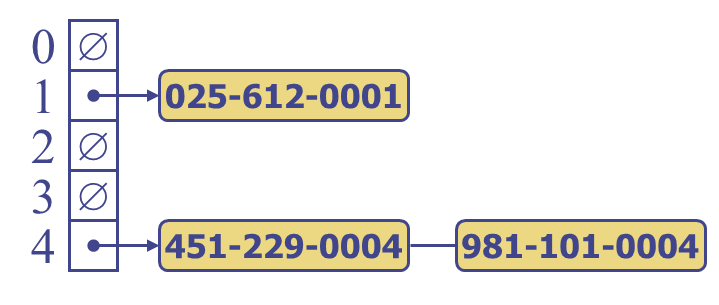
\includegraphics[width=7cm]{asp-10-pic08.png}
  \end{center}
\end{frame}

\begin{frame}[fragile,shrink]
  \frametitle{Mapa sa ulančavanjem}
  \begin{itemize}
    \item delegiramo operacije mapi implementiranoj pomoću liste za svaku ćeliju
  \end{itemize}
\begin{minted}[linenos=false]{python}
  def get(k):
    return A[h(k)].get(k)
  
  def put(k, v):
    t = A[h(k)].put(k, v)
    if t is None:
      n = n + 1
    return t
    
  def remove(k):
    t = A[h(k)].remove(k)
    if t is not None:
      n = n - 1
    return t
\end{minted}
\end{frame}

\begin{frame}[fragile,shrink=25]
  \frametitle{Heš tabela sa ulančavanjem $_1$}
\begin{minted}[linenos=false]{python}
class ChainHashMap(HashMapBase):
  """Hash map implemented with separate chaining for collision resolution."""

  def _bucket_getitem(self, j, k):
    bucket = self._table[j]
    if bucket is None:
      raise KeyError('Key Error: ' + repr(k))        # no match found
    return bucket[k]                                 # may raise KeyError

  def _bucket_setitem(self, j, k, v):
    if self._table[j] is None:
      self._table[j] = UnsortedTableMap()     # bucket is new to the table
    oldsize = len(self._table[j])
    self._table[j][k] = v
    if len(self._table[j]) > oldsize:         # key was new to the table
      self._n += 1                            # increase overall map size
\end{minted}
\end{frame}

\begin{frame}[fragile,shrink=25]
  \frametitle{Heš tabela sa ulančavanjem $_2$}
\begin{minted}[linenos=false]{python}
  def _bucket_delitem(self, j, k):
    bucket = self._table[j]
    if bucket is None:
      raise KeyError('Key Error: ' + repr(k))        # no match found
    del bucket[k]                                    # may raise KeyError

  def __iter__(self):
    for bucket in self._table:
      if bucket is not None:                         # a nonempty slot
        for key in bucket:
          yield key
\end{minted}
\end{frame}

\begin{frame}[fragile]
  \frametitle{Linearno traženje}
  \begin{itemize}
    \item \myred{linear probing}: smešta element u koliziji u prvu sledeću slobodnu ćeliju (cirkularno)
    \item elementi u koliziji se nagomilavaju izazivajući dalje kolizije
    \item primer:
%     \begin{itemize}
%       \item $h(x) = x\mod 13$
%       \item dodajemo ključeve 18, 41, 22, 44, 59, 32, 31, 73
%     \end{itemize}
  \end{itemize}
  \begin{center}
    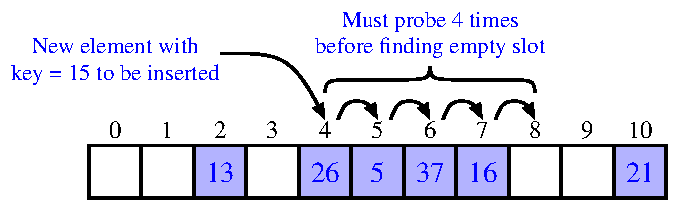
\includegraphics[width=10cm]{asp-10-pic09.pdf}
  \end{center}
\end{frame}

\begin{frame}[fragile]
  \frametitle{Čitanje sa linearnim traženjem}
  \begin{columns}
    \begin{column}[c]{6cm}
      \begin{itemize}
        \item \myred{get}(k): počinjemo od pozicije $h(k)$
        \item ispitujemo sledeće lokacije sve dok se ne dogodi nešto od:
        \begin{itemize}
          \item pronašli smo ključ $k$
          \item naišli smo na praznu lokaciju
          \item ispitali smo $N$ lokacija
        \end{itemize}
      \end{itemize}
    \end{column}
    \begin{column}[c]{5cm}
      \myred{get}($k$)
      \begin{algorithmic}
        \small
        \STATE $i \leftarrow h(k)$
        \STATE $p \leftarrow 0$
        \REPEAT
          \STATE $c \leftarrow A[i]$
          \IF{$c = \emptyset$}
            \RETURN null
          \ELSE 
            \IF{$c.getKey() = k$}
              \RETURN $c.getValue()$
            \ELSE
              \STATE $i \leftarrow (i+1)\mod N$
              \STATE $p \leftarrow p+1$
            \ENDIF
          \ENDIF
        \UNTIL{$p=N$}
        \RETURN null
      \end{algorithmic}
    \end{column}
  \end{columns}
\end{frame}

\begin{frame}[fragile]
  \frametitle{Izmene sa linearnim traženjem}
  \begin{columns}
    \begin{column}[c]{6cm}
      \begin{itemize}
        \item uvodimo poseban objekat {\tiny AVAILABLE} koji zamenjuje uklonjene elemente
        \item \myred{remove}($k$)
        \begin{itemize}
          \item tražimo element sa ključem $k$
          \item ako smo ga našli, vraćamo ga i na njegovo mesto upisujemo {\tiny AVAILABLE}
          \item inače vratimo \texttt{None}
        \end{itemize}
      \end{itemize}
    \end{column}
    \begin{column}[c]{6cm}
      \begin{itemize}
        \item \myred{put}($k, o$)
        \begin{itemize}
          \item izuzetak ako je tabela puna
          \item počinjemo od ćelije $h(k)$
          \item ispitujemo naredne ćelije sve dok se ne dogodi nešto od:
          \begin{itemize}
            \item našli smo ćeliju koja je prazna ili sadrži {\tiny AVAILABLE}
            \item isprobali smo svih $N$ ćelija
          \end{itemize}
          \item upišemo $(k, o)$ u ćeliju $i$
        \end{itemize}
      \end{itemize}
    \end{column}
  \end{columns}
\end{frame}

\begin{frame}[fragile,shrink=25]
  \frametitle{Heš tabela sa linearnim traženjem $_1$}
\begin{minted}[linenos=false]{python}
class ProbeHashMap(HashMapBase):
  """Hash map implemented with linear probing for collision resolution."""
  _AVAIL = object()       # sentinal marks locations of previous deletions

  def _is_available(self, j):
    """Return True if index j is available in table."""
    return self._table[j] is None or self._table[j] is ProbeHashMap._AVAIL

  def _find_slot(self, j, k):
    """Search for key k in bucket at index j.

    Return (success, index) tuple, described as follows:
    If match was found, success is True and index denotes its location.
    If no match found, success is False and index denotes first available slot.
    """
    firstAvail = None
    while True:                               
      if self._is_available(j):
        if firstAvail is None:
          firstAvail = j                      # mark this as first avail
        if self._table[j] is None:
          return (False, firstAvail)          # search has failed
      elif k == self._table[j]._key:
        return (True, j)                      # found a match
      j = (j + 1) % len(self._table)          # keep looking (cyclically)
\end{minted}
\end{frame}

\begin{frame}[fragile,shrink=25]
  \frametitle{Heš tabela sa linearnim traženjem $_2$}
\begin{minted}[linenos=false]{python}
  def _bucket_getitem(self, j, k):
    found, s = self._find_slot(j, k)
    if not found:
      raise KeyError('Key Error: ' + repr(k))        # no match found
    return self._table[s]._value

  def _bucket_setitem(self, j, k, v):
    found, s = self._find_slot(j, k)
    if not found:
      self._table[s] = self._Item(k,v)               # insert new item
      self._n += 1                                   # size has increased
    else:
      self._table[s]._value = v                      # overwrite existing

  def _bucket_delitem(self, j, k):
    found, s = self._find_slot(j, k)
    if not found:
      raise KeyError('Key Error: ' + repr(k))        # no match found
    self._table[s] = ProbeHashMap._AVAIL             # mark as vacated

  def __iter__(self):
    for j in range(len(self._table)):                # scan entire table
      if not self._is_available(j):
        yield self._table[j]._key
\end{minted}
\end{frame}

\begin{frame}[fragile]
  \frametitle{Duplo heširanje}
  \begin{itemize}
    \item koristi se \myred{sekundarna} heš funkcija $d(k)$
    \item prilikom kolizije element se smešta u prvu slobodnu ćeliju iz niza
    $$(i + jd(k))\mod N \quad\text{za}\,\, j = 0, 1, \ldots, N-1$$
    \item sekundarna heš funkcija ne sme vratiti 0
    \item veličina tabele $N$ mora biti prost broj da bi se mogle probati sve ćelije
    \item čest izbor za $d(k)$: \\
    $d(k) = q - (k\mod q)$
    \begin{itemize}
      \item $q < N$
      \item $q$ je prost broj
    \end{itemize}
    \item rezultat $d(k)$ je u intervalu $[1, q]$ 
  \end{itemize}
\end{frame}

\begin{frame}[fragile]
  \frametitle{Duplo heširanje: primer}
  \begin{columns}
    \begin{column}[c]{6cm}
      \begin{itemize}
        \item heš tabela sa duplim heširanjem
        \begin{itemize}
          \item $N = 13$
          \item $h(k) = k \mod 13$
          \item $d(k) = 7 - (k\mod 7)$
        \end{itemize}
        \item dodajemo ključeve 18, 41, 22, 44, 59, 32, 31, 73 
      \end{itemize}
    \end{column}
    \begin{column}[c]{6cm}
      \begin{center}
        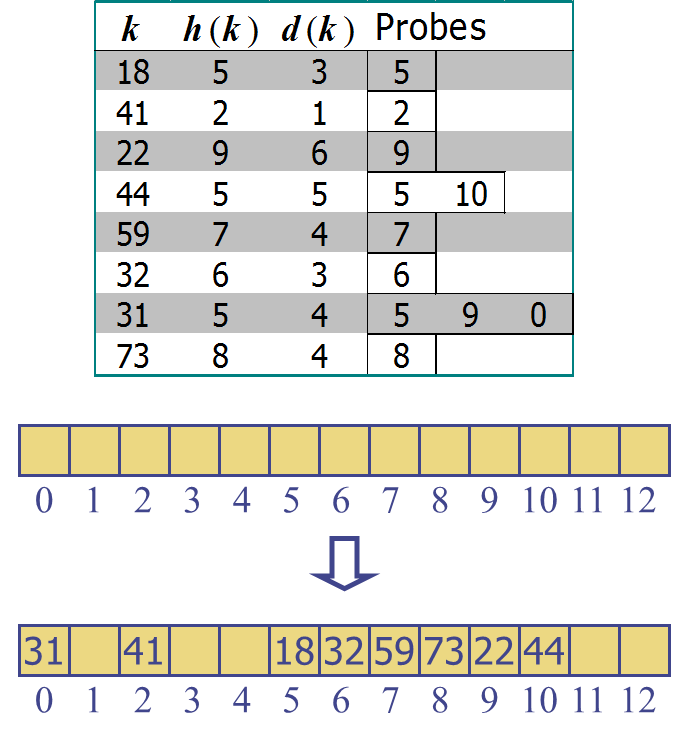
\includegraphics[width=6cm]{asp-10-pic10.png}
      \end{center}
    \end{column}
  \end{columns}
\end{frame}

\begin{frame}[fragile]
  \frametitle{Performanse heširanja}
  \begin{itemize}
    \item u najgorem slučaju pretraga, dodavanje, uklanjanje traju $O(n)$
    \item najgori slučaj: kada su \textbf{svi} ključevi u koliziji
    \item faktor popune $\alpha = n/N$ utiče na performanse
    \item ako heševi liče na slučajne brojeve može se pokazati da je očekivani broj probanja prilikom dodavanja $1/(1-\alpha)$
  \end{itemize}
\end{frame}

\begin{frame}[fragile]
  \frametitle{Performanse heširanja}
  \begin{itemize}
    \item očekivano vreme izvršavanja svih operacija je \myred{$O(1)$}
    \item u praksi heširanje je vrlo brzo ako faktor popune nije blizu 100\%
  \end{itemize}
\end{frame}

\section[Skip lista]{Skip lista}
\begin{frame}[fragile]
  \frametitle{Skip lista}
  \begin{itemize}
    \item binarna pretraga sa sortiranim nizom: omogućava pronalaženje elemenata u $O(\log n)$ vremenu
    \item ali su operacije dodavanja i uklanjanja $O(n)$ u najgorem slučaju \\ \ \\
    \item \myred{skip lista} omogućava sve u $O(\log n)$ vremenu
    \item u \textbf{prosečnom} slučaju
  \end{itemize}
\end{frame}

\begin{frame}[fragile]
  \frametitle{Skip lista}
  \begin{itemize}
    \item \myred{skip lista} za skup $S$ elemenata $(k, v)$ je serija lista $S_0, S_1, \ldots, S_h$ takvih da
    \item[1] svaka lista $S_i$ sadrži posebne ključeve $-\infty$ i $\infty$
    \item[2] lista $S_0$ sadrži ključeve iz $S$ u neopadajućem redosledu
    \item[3] svaka lista je podskup prethodne \\
    $S_0 \supseteq S_1 \supseteq \ldots \supseteq S_h$
    \item[4] lista $S_h$ sadrži samo posebne ključeve 
  \end{itemize}
  \begin{center}
    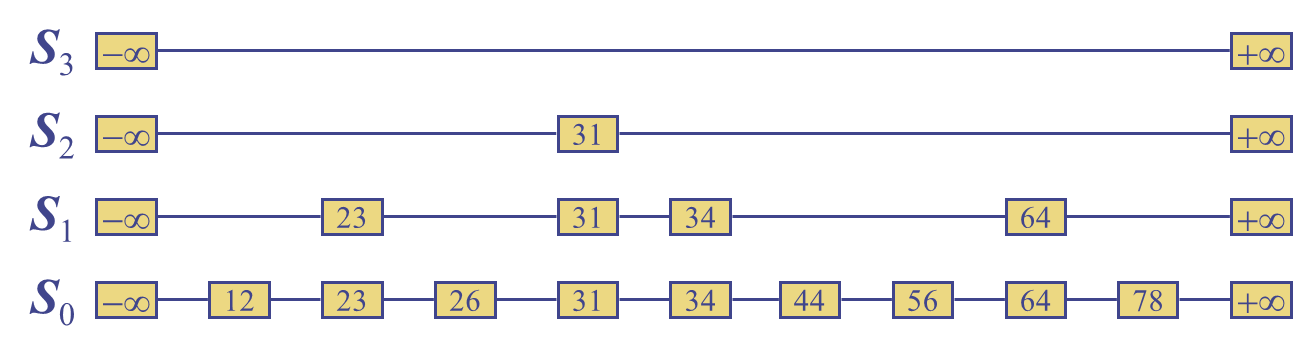
\includegraphics[width=10cm]{asp-10-pic11.png}
  \end{center}
\end{frame}

\begin{frame}[fragile]
  \frametitle{Skip lista: pretraga}
  \begin{itemize}
    \item tražimo ključ $x$ u skip listi na sledeći način:
    \item počnemo od prvog elementa liste na vrhu
    \item na tekućoj poziciji $p_i$ poredimo $x$ sa $y = key(next(p))$
    \begin{itemize}
      \item $x = y$ : pronašli smo traženi element
      \item $x > y$ : idemo napred (\myred{scan forward})
      \item $x < y$ : idemo dole (\myred{drop down})
    \end{itemize}
    \item ako smo na nivou $S_0$ i treba da idemo dole, nema traženog elementa
    \item primer: tražimo 78
  \end{itemize}
  \begin{center}
    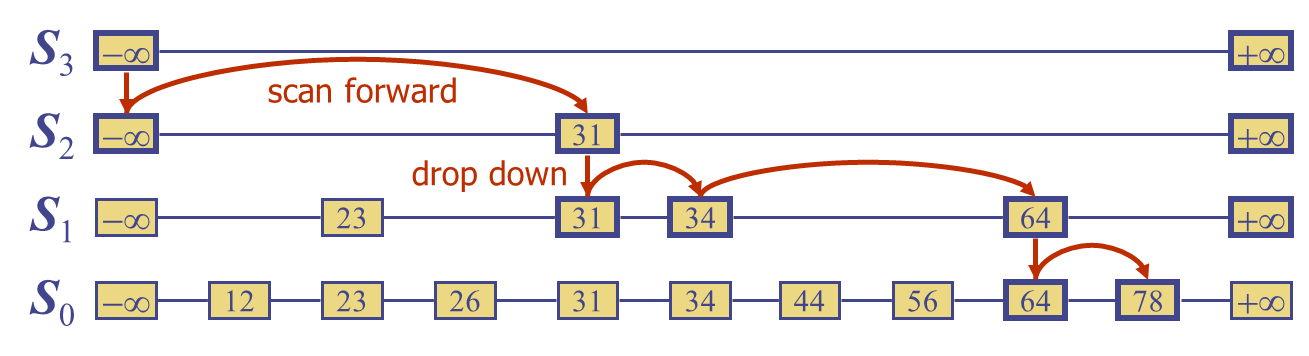
\includegraphics[width=10cm]{asp-10-pic12.png}
  \end{center}
\end{frame}

\begin{frame}[fragile]
  \frametitle{Algoritmi sa uvedenom slučajnošću}
  \begin{itemize}
    \item \myred{randomized algorithms}
    \item koriste (pseudo)slučajne vrednosti da upravlja svojim izvršavanjem
    \item sadrže naredbe nalik ovim:
    \begin{algorithmic}
      \STATE $b \leftarrow random()$
      \IF{$b = 0$}
        \STATE do A \ldots
      \ELSE
        \STATE do B \ldots
      \ENDIF
    \end{algorithmic}
    \item vreme izvršavanja zavisi od ishoda ,,bacanja novčića``
  \end{itemize}
\end{frame}

\begin{frame}[fragile]
  \frametitle{Algoritmi sa uvedenom slučajnošću}
  \begin{itemize}
    \item analiza vremena izvršavanja ovakvih algoritama podrazumeva 
    \begin{itemize}
      \item svi ishodi ,,bacanja novčića`` su jednako verovatni
      \item bacanja su međusobno nezavisna
    \end{itemize}
    \item vreme izvršavanja \textbf{u najgorem slučaju} za ovakve algoritme je često veliko ali je vrlo malo verovatno (npr. sva bacanja novčića imaju isti ishod)
    \item koristićemo ovakav algoritam za dodavanje elemenata u skip listu
  \end{itemize}
\end{frame}

\begin{frame}[fragile]
  \frametitle{Dodavanje u skip listu}
  \begin{itemize}
    \item dodavanje novog elementa $(x, o)$ u skip listu:
    \begin{itemize}
      \item ponavljamo bacanje novčića sve dok ne dobijemo ,,pismo``
      \item sa $i$ označimo broj puta koliko se pojavila ,,glava``
      \item ako je $i \geq h$ dodaćemo nove liste $S_{h+1}, \ldots, s_{i+1}$, svaku samo sa $-\infty$ + $\infty$
      \item tražimo $x$ u skip listi i nađemo pozicije $p_0, p_1, \ldots, p_i$ elemenata sa najvećim ključem manjim od $x$ u svakoj od lista $S_0, S_1, \ldots, S_i$
      \item za $j\leftarrow 0, \ldots, i$ dodaćemo $(x, o)$ u listu $S_j$ nakon pozicije $p_j$
    \end{itemize}
    \item primer: dodajemo ključ 15, za $i=2$ 
  \end{itemize}
  \begin{center}
    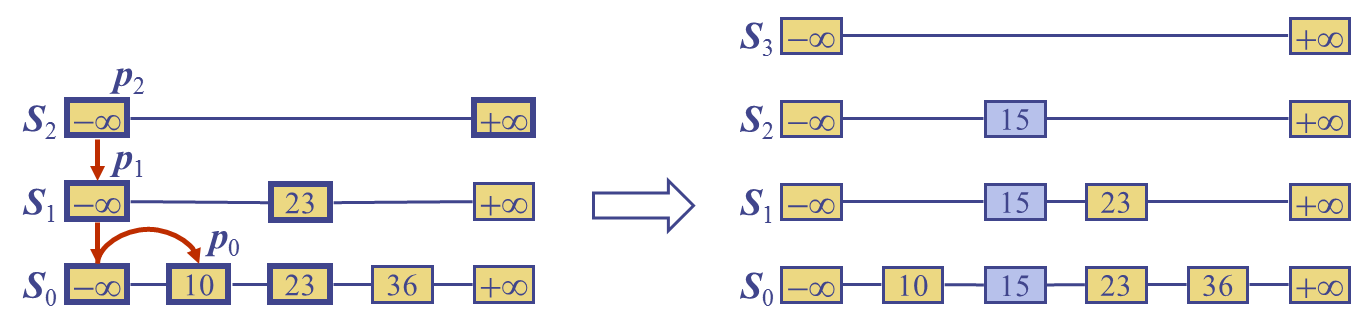
\includegraphics[width=11cm]{asp-10-pic13.png}
  \end{center}
\end{frame}

\renewcommand{\algorithmiccomment}[1]{\hfill \{\myred{#1}\}}

\begin{frame}[fragile,shrink]
\frametitle{Dodavanje u skip listu}
\myred{SkipInsert}($k, v$)
\begin{algorithmic}
\REQUIRE ključ $k$ i vrednost $v$
\ENSURE najviša pozicija dodatog elementa
\STATE $p \leftarrow$ SkipSearch(k)
\STATE $q \leftarrow$ None \COMMENT{$q$ će biti najviši čvor u koloni novog elementa}
\STATE $i \leftarrow -1$
\REPEAT
  \STATE $i\leftarrow i+1$
  \IF{$i\geq h$}
    \STATE $h \leftarrow h + 1$ \COMMENT{dodajemo novi nivo u skip listu}
    \STATE $t \leftarrow$ next($s$)
    \STATE $s \leftarrow$ insertAfterAbove(None, $s$, ($-\infty$, None)) \COMMENT{povećaj levu}
    \STATE insertAfterAbove(s, t, ($+\infty$, None)) \COMMENT{povećaj desnu kulu}
  \ENDIF
  \WHILE{above(p) is None}
    \STATE $p \leftarrow$ prev($p$) \COMMENT{idi nazad}
  \ENDWHILE
  \STATE $p \leftarrow$ above($p$) \COMMENT{popni se 1 nivo}
  \STATE $q \leftarrow$ insertAfterAbove($p,q,(k,v)$) \COMMENT{povećaj visinu kule}
\UNTIL{coinFlip()==tails}
\STATE $n \leftarrow n + 1$
\RETURN $q$
\end{algorithmic}
\end{frame}

\begin{frame}[fragile]
  \frametitle{Uklanjanje iz skip liste}
  \begin{itemize}
    \item uklanjanje elementa sa ključem $x$ iz skip liste:
    \begin{itemize}
      \item tražimo $x$ u skip listi i nađemo pozicije $p_0, p_1, \ldots, p_i$ elemenata sa najvećim ključem manjim od $x$ u svakoj od lista $S_0, S_1, \ldots, S_i$
      \item uklonimo pozicije $p_0, p_1, \ldots, p_i$ iz listi
      \item uklonimo sve prazne liste osim jedne
    \end{itemize}
    \item primer: uklanjamo ključ 34 
  \end{itemize}
  \begin{center}
    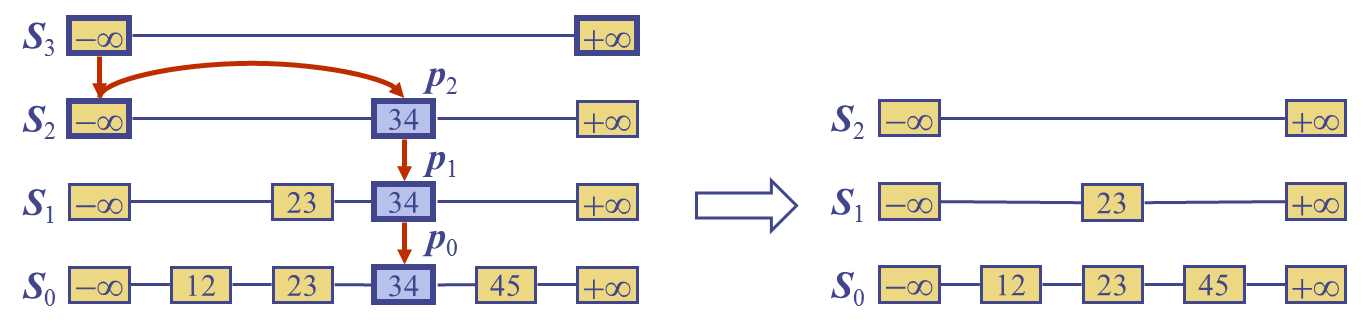
\includegraphics[width=11cm]{asp-10-pic14.png}
  \end{center}
\end{frame}

\begin{frame}[fragile]
  \frametitle{Implementacija skip liste}
  \begin{columns}
    \begin{column}[c]{6cm}
      \begin{itemize}
        \item možemo da koristimo \myred{quad-nodes}
        \begin{itemize}
          \item element
          \item link na prethodni
          \item link na sledeći
          \item link na čvor ispod
          \item link na čvor iznad
        \end{itemize}
        \item definišemo specijalne ključeve {\tiny PLUS\_INF} i {\tiny MINUS\_INF} i odgovarajući komparator 
      \end{itemize}
    \end{column}
    \begin{column}[c]{6cm}
      \begin{center}
        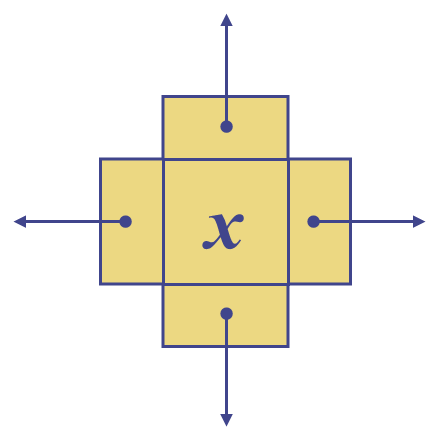
\includegraphics[width=5cm]{asp-10-pic15.png}
      \end{center}
    \end{column}
  \end{columns}
\end{frame}

\begin{frame}[fragile]
  \frametitle{Skip liste i zauzeće prostora}
  \begin{itemize}
    \item količina zauzete memorije zavisi od bacanja novčića
    \item iz teorije verovatnoće
    \begin{itemize}
      \item[(a)] verovatnoća da se dobije $i$ uzastopnih glava je $1/2^i$
      \item[(b)] ako je svaki od $n$ elemenata prisutan u listi sa verovatnoćom $p$, veličina skupa je $np$
      \item[(c)] ako svaki od $n$ događaja ima verovatnoću $p$, verovatnoća da će se desiti bar jedan nije veća od $np$
      \item[(d)] očekivani broj bacanja novčića da se dobije ,,pismo`` je 2
    \end{itemize}
  \end{itemize}
\end{frame}

\begin{frame}[fragile]
  \frametitle{Skip liste i zauzeće prostora}
  \begin{itemize}
    \item posmatramo skip listu sa $n$ elemenata
    \begin{itemize}
      \item prema (a), dodaćemo čvor u listu $S_i$ sa verovatnoćom $1/2^i$
      \item prema (b), očekivana veličina liste $S_i$ je $n/2^i$
    \end{itemize}
    \item očekivani broj čvorova u skip listi je
    $$ \sum_{i=0}^h \frac{n}{2^i} = n \sum_{i=0}^h \frac{1}{2^i} < 2n$$
    \item prema tome, očekivani broj čvorova u skip listi sa $n$ elemenata je \myred{$O(n)$}
  \end{itemize}
\end{frame}

\begin{frame}[fragile]
  \frametitle{Visina skip liste}
  \begin{itemize}
    \item vreme izvršavanja pretrage i dodavanja u skip listu zavisi od njene \textbf{visine}
    \item posmatramo skip listu sa $n$ elemenata
    \begin{itemize}
      \item prema (a), dodaćemo čvor u listu $S_i$ sa verovatnoćom $1/2^i$
      \item prema (c), verovatnoća da $S_i$ ima bar jedan čvor je najviše $n/2^i$
    \end{itemize}
    \item ako izaberemo $i=3\log n$, verovatnoća da $S_{3\log n}$ ima bar jedan čvor je najviše
    $$\frac{n}{2^{3\log n}} = \frac{n}{n^3} = \frac{1}{n^2}$$
    \item prema tome, skip lista sa $n$ elemenata je visoka najviše $3\log n$ sa verovatnoćom najmanje $1-1/n^2$
  \end{itemize}
\end{frame}

\begin{frame}[fragile]
  \frametitle{Visina skip liste}
  \begin{itemize}
    \item sa vrlo velikom verovatnoćom
    \item visina skip liste sa $n$ elemenata je $O(\log n)$
  \end{itemize}
\end{frame}

\begin{frame}[fragile]
  \frametitle{Pretraga i ažuriranje skip liste}
  \begin{itemize}
    \item vreme pretrage je proporcionalno
    \begin{itemize}
      \item broju \myred{drop down} koraka, plus
      \item broju \myred{scan forward} koraka
    \end{itemize}
    \item drop down koraci su ograničeni visinom skip liste, dakle $O(\log n)$ sa velikom verovatnoćom
  \end{itemize}
\end{frame}

\begin{frame}[fragile]
  \frametitle{Pretraga i ažuriranje skip liste}
  \begin{itemize}
    \item kada radimo \myred{scan forward} korak, ključ se ne nalazi u listi iznad
    \begin{itemize}
      \item scan forward postoji zato što je ranije novčić dao ,,pismo``
    \end{itemize}
    \item prema (d), u svakoj listi očekivani broj scan forward koraka je 2
    \item prema tome, ukupan broj scan forward koraka je $O(\log n)$
    \item očekivano vreme za pretragu u skip listi je \myred{$O(\log n)$}
    \item slično tome dodavanje i uklanjanje
  \end{itemize}
\end{frame}

\begin{frame}[fragile]
  \frametitle{Performanse skip liste}
  \begin{itemize}
    \item skip lista je struktura podataka za implementaciju mape
    \item upotreba memorije je $O(n)$
    \item brzina pretrage, dodavanja i uklanjanja je $O(\log n)$ sa velikom verovatnoćom
  \end{itemize}
\end{frame}

\section[Skup]{Skup}
\begin{frame}[fragile]
  \frametitle{Skup, multiskup, multimapa}
  \begin{itemize}
    \item \myred{skup} (set) je kolekcija elemenata koja ne poznaje redosled i ne sadrži duplikate
    \begin{itemize}
      \item elementi skupa su nalik ključevima koji nemaju sebi asocirane vrednosti
    \end{itemize}
    \item \myred{multiskup} (multiset, \myred{bag}) je skup koji dopušta duplikate
    \item \myred{multimapa} je mapa koja dopušta da za jedan ključ bude vezano više vrednosti
    \begin{itemize}
      \item indeks u knjizi preslikava pojam na jednu ili više stranica na kojima se on pominje
    \end{itemize}
  \end{itemize}
\end{frame}

\begin{frame}[fragile]
  \frametitle{Skup ATP: osnovne operacije}
  \begin{center}
    \begin{tabular}{rp{8cm}}
      \textbf{\texttt{S.add(e)}} & dodaje element $e$ u $S$; nema efekta ako je $e$ već prisutan u $S$\\ \hline
      \textbf{\texttt{S.discard(e)}} & uklanja $e$ iz $S$; nema efekta ako $e$ nije prisutan u $S$\\ \hline
      \textbf{\texttt{e in S}} & vraća \texttt{True} ako je $e$ prisutan u $S$; implementira je \texttt{\_\_contains\_\_} \\ \hline
      \textbf{\texttt{len(S)}} & vraća broj elemenata u $S$; implementira je \texttt{\_\_len\_\_} \\ \hline
      \textbf{\texttt{iter(S)}} & iterira kroz elemente iz $S$; implementira je \texttt{\_\_iter\_\_} \\
    \end{tabular}
  \end{center}
  \begin{itemize}
    \item pomoću osnovnih operacija implementiraju se sve ostale
  \end{itemize}
\end{frame}

\begin{frame}[fragile]
  \frametitle{Skup ATP: dodatne operacije}
  \begin{center}
    \begin{tabular}{rp{8cm}}
      \textbf{\texttt{S.remove(e)}} & uklanja $e$ iz $S$; ako $e$ nije prisutan u $S$ izaziva \texttt{KeyError}\\ \hline
      \textbf{\texttt{S.pop()}} & vraća i uklanja proizvoljan element iz $S$; ako je $S$ prazan izaziva \texttt{KeyError}\\ \hline
      \textbf{\texttt{S.clear()}} & uklanja sve elemente iz $S$ \\
    \end{tabular}
  \end{center}
\end{frame}

\begin{frame}[fragile]
  \frametitle{Skup ATP: poređenje skupova}
  \begin{center}
    \begin{tabular}{rp{7.5cm}}
      \textbf{\texttt{S == T}} & vraća \texttt{True} ako skupovi imaju jednak sadržaj \\ \hline
      \textbf{\texttt{S != T}} & vraća \texttt{True} ako skupovi nemaju jednak sadržaj \\ \hline
      \textbf{\texttt{S <= T}} & vraća \texttt{True} ako je $S$ podskup od $T$ \\ \hline
      \textbf{\texttt{S < T}} & vraća \texttt{True} ako je $S$ pravi podskup od $T$ \\ \hline
      \textbf{\texttt{S >= T}} & vraća \texttt{True} ako je $S$ nadskup od $T$ \\ \hline
      \textbf{\texttt{S > T}} & vraća \texttt{True} ako je $S$ pravi nadskup od $T$ \\ \hline
      \textbf{\texttt{S.isdisjoint(T)}} & vraća \texttt{True} ako su $S$ i $T$ disjunktni \\
    \end{tabular}
  \end{center}
\end{frame}

\begin{frame}[fragile]
  \frametitle{Skup ATP: operacije nad skupovima}
  \begin{center}
    \begin{tabular}{cp{8.5cm}}
      \textbf{\texttt{S | T}} & vraća novi skup koji je unija $S$ i $T$ \\ \hline
      \textbf{\texttt{S |= T}} & ažurira $S$ da bude unija $S$ i $T$ \\ \hline
      \textbf{\texttt{S \& T}} & vraća novi skup koji je presek $S$ i $T$ \\ \hline
      \textbf{\texttt{S \&= T}} & ažurira $S$ da bude presek $S$ i $T$ \\ \hline
      \textbf{\texttt{S \^{} T}} & vraća simetričnu razliku $S$ i $T$ \\ \hline
      \textbf{\texttt{S \^{}= T}} & ažurira $S$ da bude simetrična razlika $S$ i $T$ \\ \hline
      \textbf{\texttt{S - T}} & vraća razliku $S$ i $T$ \\ \hline
      \textbf{\texttt{S -= T}} & ažurira $S$ da bude razlika $S$ i $T$ \\
    \end{tabular}
  \end{center}
\end{frame}

\begin{frame}[fragile,shrink]
  \frametitle{Implementacija skupa: poređenje $S < T$}
\begin{minted}[linenos=false]{python}
def __lt__(self, other):
  """Vraća True ako je self pravi podskup od other."""
  if len(self) >= len(other):
    return False  # pravi podskup mora biti manji
  for e in self:
    if e not in other:
      return False  # nije podskup, fali mu e
  return True
  \end{minted}
\end{frame}

\begin{frame}[fragile,shrink]
  \frametitle{Implementacija skupa: unija $S | T$}
\begin{minted}[linenos=false]{python}
def __or__(self, other):
  """Vraća novi skup kao uniju self i other."""
  result = Set()  # rezultat je nova instanca
  for e in self:
    result.add(e)
  for e in other:
    result.add(e)
  return result
\end{minted}
\end{frame}

\begin{frame}[fragile,shrink]
  \frametitle{Implementacija skupa: operacija $S |= T$}
\begin{minted}[linenos=false]{python}
def __ior__(self, other):
  """Menja self da bude unija self i other."""
  for e in other:
    self.add(e)
  return self   # mora da se vrati self za operator |=
\end{minted}
\end{frame}

\begin{frame}[fragile]
  \frametitle{Implementacija skupa: struktura podataka}
  \begin{itemize}
    \item pomoću liste
    \item upotreba memorije je $O(n)$
    \item \texttt{\_\_contains\_\_} je $O(n)$
  \end{itemize} 
  \begin{center}
    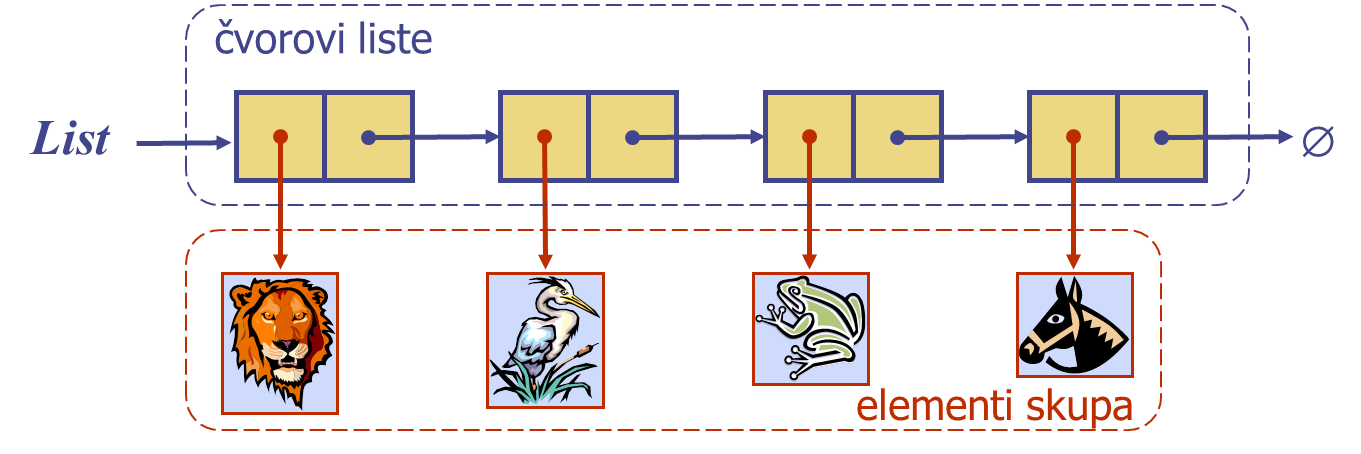
\includegraphics[width=10cm]{asp-10-pic16.png}
  \end{center}
\end{frame}

\begin{frame}[fragile]
  \frametitle{Implementacija skupa: struktura podataka}
  \begin{itemize}
    \item pomoću hash tabele
    \item hash tabela čuva samo ključeve tj. elemente
    \item \texttt{\_\_contains\_\_} je $O(1)$ \\ \ \\
    \item za koje vreme rade presek i unija?
  \end{itemize} 
\end{frame}

\end{document}
